\section{Scenarios}
\begin{frame}{Scenarios}
rootJS is used by applications to access the ROOT framework\\
\pause $\Rightarrow $ our users are those applications
\end{frame}

\subsection{Event Viewer}
\begin{frame}{Event Viewer}
 \pause   Event Viewers provide visualisation of experimental data
  \begin{itemize}
    \pause \item useful for quick eyescan of data
    \pause \item check if data is recorded properly
  \end{itemize}
  \pause
  \medskip
   \begin{figure}[htb]
      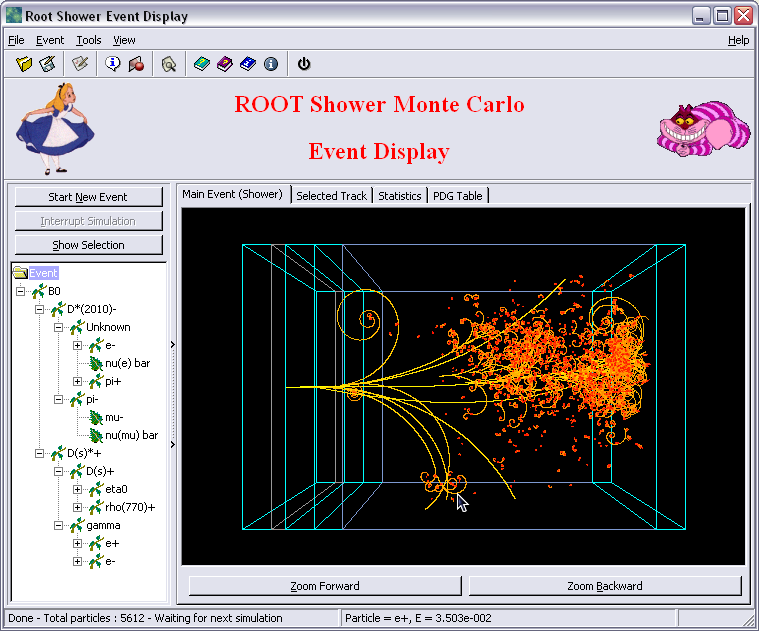
\includegraphics[width=0.6\linewidth, keepaspectratio]{./resources/shower_event_viewer.png}
      \nocite{cern:root:eventviewer}
   \end{figure}
   \end{frame}

\begin{frame}{Event Viewer}
   Conventional ROOT Event Viewer
  \begin{itemize}
  \pause \item standalone ROOT application
   \pause \item requires ROOT on machine
   \pause \item requires ROOT's dependencies
   \pause \item requires access to data source
   \end{itemize}
   \pause $\Rightarrow $ very limited portability and harsh requirements for client system
\end{frame}

\begin{frame}{Event Viewer}
 Client/Server based Web Event Viewer using rootJS and nodeJS
  \begin{itemize}
  \pause \item server runs ROOT and its dependencies
   \pause \item no access to critical data sources required
   \pause \item no heavy work load on client system
   \pause \item client only needs modern web browser
   \end{itemize}

   \pause $\Rightarrow $ great portability and ease of use as client can be almost any device
\end{frame}

\begin{frame}{Event Viewer}
  \begin{longtable}{p{3cm} @{\hskip 0.7cm} p{7cm}}
    \hline
    \textit{Scenario name} & \texttt{EventViewer}\\
    \hline
    \hline
    \textit{Participating actors} &
    \underline{Server:EventViewerServer}; \underline{:ROOT}\\
    & \underline{Client:EventViewerClient}; \underline{:rootJS}\\
    \hline
    \textit{Flow of events} &
    \begin{itemize}
      \setlength{\itemindent}{-2em}
      \item \texttt{Client} requests updates from \texttt{Server}.
      \item \texttt{Server} interfaces with \texttt{ROOT} through 
      \\\hspace{-2em}\texttt{rootJS}.
      \item \texttt{ROOT}'s I/O accesses and processes data
      \item \texttt{ROOT} returns the data to the \texttt{Server} using 
      \\\hspace{-2em}\texttt{rootJS}.
      \item \texttt{Server} sends the data to the \texttt{Client} 
      \item \texttt{Client} renders data locally.
    \end{itemize}
  \end{longtable}
\end{frame}


\begin{frame}{Scenarios}
  In what ways could these bindings also improve work efficiency for scientists?
  \begin{itemize}
  \pause \item integrating run logs and quality assurance in ROOT workflow
  \pause \item ...
  \end{itemize}
\end{frame}